\documentclass[orange]{../LaTeX-Templates/Skript/skript}

\title{Theoretische Informatik\\\subtitleformat{Zusammenfassung der Module TI 1 und 2}}
\author{Simon \textsc{König}}

\usepackage{pgf}
\usepackage{tikz}
\usetikzlibrary{arrows,automata,positioning,trees, shapes}

\newcommand{\re}{\mathrm{(r.e.)}}
\newcommand{\rec}{\mathrm{(REC)}}
\newcommand{\csl}{\mathrm{(CSL)}}
\newcommand{\cfl}{\mathrm{(CFL)}}
\newcommand{\dcfl}{\mathrm{(DCFL)}}
\newcommand{\reg}{\mathrm{(REG)}}
\newcommand{\fin}{\mathrm{(FIN)}}

\newcommand{\poly}{\textbf{P}}
\newcommand{\npoly}{\textbf{NP}}

\renewcommand{\version}{\today}

\begin{document}
\maketitle
\tableofcontents



\chapter{Überblick}
Ein kurzer Gesamtüberblick über den Zusammenhang von formalen Sprachen zur Komplexität und Berechenbarkeitstheorie:

\definecolor{entscheidbar}{rgb}{0.4, 0.9, 0.7}
	\begin{center}
		\begin{tikzpicture}
			\tikzset{
			grouplabel/.style={
			draw,
			fill = white,
			rectangle,
			inner sep = 4pt,
			rounded corners=1pt
			}
			}

			\draw [rounded corners=5pt, dotted, line width=0.2mm] (0,0) rectangle (14,16.5);
			\draw node at (7,16.5) [grouplabel] {alle formalen Sprachen};


			% CO-SEMI-ENTSCHEIDBAR
			\draw [rounded corners=5pt, dotted, line width=0.5mm] (0.5,0.5) rectangle (12,12);%co-semi
			\draw node at (6,0.5) [grouplabel] {co-semi-entscheidbare Sprachen};
			\draw node at (0.5,1.3) [label={right:$\chi'_{\overline L}(w)$ ist Turing-berechenbar, Komplement ist semi-entscheidbar}] {};

			% SEMI-ENTSCHEIDBAR
			\draw [rounded corners=5pt, dotted, line width=0.5mm] (2,2) rectangle (13.5,15.5);%semi
			\draw node at (8,15.5) [grouplabel] {\hyperref[sec:typ0]{$\operatorname{Typ-0}=\re$, semi-entscheidbare Sprachen}};
			\draw node at (2,14.8) [label={right:$\operatorname{PCP, K, H, H_0, \ldots}$}] {};
			\draw node at (2,14.3) [label={right:$\chi'_{L}(w)$ ist Turing-berechenbar}] {};
			\draw node at (2,13.7) [label={right:$L=T(M) \rightsquigarrow$ wird durch eine TM akzeptiert}] {};
			\draw node at (2,13.2) [label={right:$f:\N\rightarrow \Sigma^\star, f(\N)=L \rightsquigarrow$ rekursiv aufzählbar}] {};
			\draw node at (2,12.7) [label={right:$f:\Sigma^\star\rightarrow\Sigma^\star, f(\Sigma^\star)=L \rightsquigarrow$ Wertebereich einer berechenbaren Funktion}] {};


			%ENTSCHEIDBAR
			\draw [draw, fill=accent!50, line width=0.5mm] (2,2) rectangle (12,12);%entscheidbar
			\draw node at (7,12) [grouplabel] {\hyperref[sec:rec]{entscheidbare Sprachen}};
			\draw node at (2,10.5) [label={right:$\chi_{L}(w)$ ist Turing-berechenbar}] {};



			%% TYP1
			\draw [rounded corners=2pt, line width=0.2mm] (2.2,2.2) rectangle (11.8,9.9);
			\draw node at (7,9.9) [grouplabel] {\hyperref[sec:typ1]{$\operatorname{Typ-1}=\csl$}};
			\draw node at (2.2,9.2) [label={right:$a^nb^nc^n, a^{2^n}, \ldots$}] {};
			\draw node at (2.2,8.7) [label={right:LBA}] {};

			%% TYP2
			\draw [rounded corners=2pt, line width=0.2mm] (2.4,2.4) rectangle (11.6,8.1);
			\draw node at (7,8.1) [grouplabel] {\hyperref[sec:typ2]{$\operatorname{Typ-2}=\cfl$}};
			\draw node at (2.4,7.4) [label={right:$a^na^n, ww^R, \ldots$}] {};
			\draw node at (2.4,6.9) [label={right:PDA}] {};

			% DCFL
			\draw [rounded corners=2pt, line width=0.2mm] (2.6,2.6) rectangle (11.4,6.3);%dcfl
			\draw node at (7,6.3) [grouplabel] {\hyperref[sec:typ2]{$\dcfl$}};
			\draw node at (2.6,5.6) [label={right:$a^nb^n, w\$w^R, \ldots$}] {};
			\draw node at (2.6,5.1) [label={right:DPDA}] {};

			% TYP3
			\draw [rounded corners=2pt, line width=0.2mm] (2.8,2.8) rectangle (11.2,4.5);
			\draw node at (7,4.5) [grouplabel] {\hyperref[sec:typ3]{$\operatorname{Typ-0}=\reg$}};
			\draw node at (2.8,3.8) [label={right:$\Sigma^\star, \emptyset, a^\star,\ldots$}] {};
			\draw node at (2.8,3.3) [label={right:DEA, NEA, reguläre Ausdrücke}] {};

			\draw node at (14.1,0.2) [label={left:{\color{black!50!white}Simon König 2018}}] {};

		\end{tikzpicture}
	\end{center}


\part{Grundlagen}
	\chapter{Grundlagen der Aussagenlogik}
\section{Syntax der Aussagenlogik}
\begin{itemize}
	\item Atomare Formeln: $A_i$ mit $i\in\N$
	\item $F$ und $G$ Formeln $\rightarrow$ $(F\wedge G)$, $(F\vee G)$ und $\neg F$ auch Formeln
\end{itemize}
\section{Semantik der Aussagenlogik}
$D\subseteq\simpleset{A_1,A_2,\ldots}$

Eine Abbildung $\mathcal A:D\rightarrow\simpleset{0,1}$ heißt Belegung.
Weiter

\begin{itemize}
	\item Eine Belegung $\mathcal A$ ist \textbf{passend} zu einer  Formel $F$, falls alle in $F$ vorkommenden atomaren Variablen zum Definitionsbereich von $\mathcal A$ gehören.
	\item Eine Belegung $\mathcal A$ ist \textbf{Modell} für eine Formel, falls $\mathcal A$ zu $F$ passend ist und $\mathcal A(F)=1$ gilt.\\
			Man schreibt dann $\mathcal A \vDash F$.
	\item $F$ ist \textbf{erfüllbar}, falls ein Modell für $F$ existiert.
	\item $F$ ist \textbf{gültig}, falls alle passenden Belegungen Modelle sind. $\rightarrow$ $F$ nennt man dann eine  \textbf{Tautologie}. Das Komplement einer Tautologie ist unerfüllbar.
	\item Zwei Formeln $F$ und $G$ heißen \textbf{semantisch äquivalent}, wenn alle zu beiden passenden Belegungen $\mathcal A$ gilt: $\mathcal A(F) = \mathcal A(G)$. Man schreibt dann $F\equiv G$.
\end{itemize}

\section{Prädikatenlogik}

\part{Formale Sprachen und Automatentheorie}
	\chapter{Einstieg}
In der Theorie um formale Sprachen geht es grundsätzlich darum, Probleme durch formale Sprachen beschreiben zu können. Diese Probleme werden dann in Klassen eingeordnet und gegeneinander abgregrenzt. Wichtig ist zu verstehen, wie man eine formale Sprache beschreiben kann und wo die Unterschiede zwischen den Klassen liegen.


	\chapter{Endliche Sprachen}
\begin{equation*}
	\fin\subset\reg\subset\dcfl\subset\cfl\subset\csl\subset\rec\subset\re
\end{equation*}
Alle endlichen Sprachen sind regulär.

\section{Beispiele}
\begin{itemize}
	\item $L_1=\emptyset$ (leere Sprache ist endlich)
	\item $L_2=\Sigma$ (nur die Buchstaben)
	\item $L_3=\simpleset{aaa,baba}$ (z.B. nur zwei Wörter)
\end{itemize}

	\chapter{Reguläre Sprachen}
\begin{equation*}
	\text{Typ-3} = \reg\subset\dcfl\subset\cfl\subset\csl\subset\rec\subset\re
\end{equation*}

\section{Automatenmodell DEA}
Ein deterministischer endlicher Automat ist ein 5-Tupel
\begin{equation*}
	M=(Z,\Sigma,\delta,z_0,E)
\end{equation*}
\begin{description}
	\item[$Z$] endliche Zustandsmenge
	\item[$\Sigma$] Eingabealphabet
	\item[$\delta$] Überführungsfunktion $\delta:Z\times\Sigma\rightarrow Z$
	\item[$z_0$] Startzustand, $z_0\in Z$
	\item[$E$] Endzustandsmenge, $E\subseteq Z$
\end{description}
\bigskip
Es lässt sich außerdem eine erweiterte Funktion $\hat\delta$ definieren:
\begin{align*}
	&\hat\delta:Z\times\Sigma^\star\rightarrow Z\\
	\intertext{Mit den folgenden Eigenschaften:}
	&\hat\delta(z,\epsilon)=z\\
	&\hat\delta(z,ax)=\hat\delta(\delta(z,a),x)
\end{align*}
Die von einem deterministischen Automaten $M$ akzeptierte Sprache ist
\begin{equation*}
	T(M)=\set{w\in\Sigma^\star}{\hat\delta(z_0,w)\in E}
\end{equation*}

\section{Automatenmodell NEA}\label{reg:nea}
Ein nichtdeterministischer endlicher Automat ist ein 5-Tupel
\begin{equation*}
	M=(Z,\Sigma,\delta,S,E)
\end{equation*}
\begin{description}
	\item[$Z$] endliche Zustandsmenge
	\item[$\Sigma$] Eingabealphabet
	\item[$\delta$] Überführungsfunktion $\delta:Z\times\Sigma\rightarrow \Pot(Z)$
	\item[$S$] Startzustandsmenge, $S\subseteq Z$
	\item[$E$] Endzustandsmenge, $E\subseteq Z$
\end{description}
Der NEA ist formal stärker als der DEA, sie akzeptieren jedoch beide die selbe Sprachklasse.

Die akzeptierte Sprache eines nichtdeterministischen endlichen Automaten ist:
\begin{equation*}
	T(M)=\set{w\in\Sigma^\star}{\hat\delta(S,w)\cap E\neq \emptyset}
\end{equation*}

\section{Reguläre Ausdrücke}
Die regulären Sprachen lassen sich zusätzlich zu den zwei Automatenmodellen auch durch sog. reguläre Ausdrücke beschreiben. Eine Definition für die Syntax der regulären Ausdrücke ist:
\begin{itemize}
	\item $\emptyset$ und $\epsilon$ sind reguläre Ausdrücke.
	\item $a$ ist ein regulärer Ausdruck für alle $a\in\Sigma$
	\item Wenn $\alpha$ und $\beta$ eguläre Ausdrücke sind, dann sind auch $\alpha\beta$, $(\alpha|\beta)$ und $(\alpha)^\star$ reguläre Ausdrücke.
\end{itemize}
Die Semantik der regulären Ausdrücke ist ebenso induktiv bestimmt:
\begin{itemize}
	\item $L(\emptyset)=\emptyset$ und $L(\epsilon)=\simpleset{\epsilon}$
	\item $L(a)=\simpleset{a}$ für jedes $a\in\Sigma$
	\item $L(\alpha \beta)=L(\alpha)L(\beta)$, $L(\alpha|\beta)=L(\alpha)\cup L(\beta)$, $L((\alpha)^\star)=L(\alpha)^\star$
\end{itemize}






\section{Sätze zu den regulären Sprachen:}
\begin{itemize}
	\item Typ-3 Sprachen können \emph{nicht} inhärent mehrdeutig sein, da sich zu jeder Sprache ein Minimalautomat bilden lässt.
	\item Die Klasse der Typ-3 Sprachen ist unter allen boole'schen Operationen, Sternoperation und der Konkatenation abgeschlossen.
	\item Für reguläre Sprachen ist das Wortproblem (in Linearzeit), das Leerheitsproblem, das Äquivalenzproblem sowie das Schnittproblem entscheidbar.
	\item Alle Typ-2 Sprachen über einem einelementigen Alphabet sind bereits regulär.
\end{itemize}
\subsection{Pumping-Lemma für Typ-3}%
	Für jede reguläre Sprache $L$ gibt es ein $n\in\N$, so dass für jedes $x\in L$ mit $|x|\geq n$ eine Zerlegung in drei Teile exisitert: $x=uvw$, so dass die drei Bedingungen erfüllt sind:
	\begin{itemize}
		\item $|v|\geq 1$
		\item $|uv|\leq n$
		\item $\forall i \in\N: uv^iw\in L$ (\glqq Pump-Bedingung\grqq)
	\end{itemize}
	\begin{align*}
		\intertext{Gilt die Negation dieser Aussage, also}
		\forall n\in\N:\exists x\in L, |x|\geq n : \forall u,v,w \in\Sigma^\star, x=uvw, |v|\geq 1, |uv|\leq n:\exists i\in\N:uv^iw\not\in L
		\intertext{so ist L nicht regulär!}
 	\end{align*}%

	\textbf{ABER:} Das Pumping-Lemma gibt keine Charakterisierung der Typ-3 Sprachen an! Es gibt auch Sprachen, die nicht Typ-3 sind, die Aussage des Lemmas aber trotzdem erfüllen!

	Das Pumping-Lemma gibt also nur eine Möglichkeit, zu Beweisen, dass eine Sprache \emph{nicht} regulär ist! (Siehe \autoref{bsp:pumpingLemma})
\subsection{Myhill-Nerode-Äquivalenz}%
	Mit der Myhill-Nerode-Äquivalenz ist es möglich nachzuweisen, ob eine Sprache regulär ist.
	\begin{align*}
		&x \mathrm R_L y \Longleftrightarrow \left[\forall w\in\Sigma^\star : xw\in L \Leftrightarrow yw\in L\right]\\
		\intertext{Bzw. anhand eines DEA (dies führt zu einer Verfeinerung von $\mathrm R_L$)}
		&x \mathrm R_M y \Longleftrightarrow \left[\delta (z_0,x)=\delta (z_0,y)\right]\\
		\intertext{Es gilt:}
		&x \mathrm R_M y \Rightarrow \forall w\in\Sigma^\star : \delta (z_0,xw)=\delta (z_0,yw) \Rightarrow x \mathrm R_L y
	\end{align*}
	Die Sprache $L\subseteq \Sigma^\star$ ist genau dann regulär, wenn der Index der Myhill-Nerode-Äquivalenz $\mathrm R_L$endlich ist.


\subsection{Erkennung durch Monoide -- Syntaktisches Monoid}
	Sei $L\subseteq \Sigma^\star$ eine formale Sprache und $M$ ein Monoid.

	$M$ erkennt $L$, wenn eine Teilmenge $A\subseteq M$ und ein Homomorphismus $\varphi:\Sigma^\star \rightarrow M$ existiert, so dass gilt:
	\begin{align*}
		L&=\varphi^{-1}(A) &&\text{d.h. }w\in L \Leftrightarrow \varphi(w)\in A\\
		L&=\varphi^{-1}(\varphi(L)) &&\text{d.h. }w\in L \Leftrightarrow \varphi(w)\in \varphi(L)
	\end{align*}

	Weiter kann man für eine konkrete Sprache $L$ die \emph{syntaktische Kongruenz} definieren:
	\begin{align*}
		w_1\equiv_Lw_2 \Longleftrightarrow [\forall x,y\in\Sigma^\star : xw_1y\in L \Leftrightarrow xw_2y\in L]
	\end{align*}

	Basierend auf dieser Kongruenz definieren wir das Quotientenmonoid der Kongruenz, dessen Elemente die Äquivalenzklassen sind.

	Das Quotientenmonoid oder auch syntaktisches Monoid bezüglich der syntaktischen Kongruenz wird mit
	\begin{equation*}
		\mathrm{Synt}(L)\coloneqq\left(\Sigma^\star/\equiv_L\right)
	\end{equation*}
	bezeichnet.

	Für jede Sprache $L$ gibt es ein syntaktisches Monoid das $L$ mit dem Homomorphismus
	\begin{equation*}
		\varphi: L\rightarrow \mathrm{Synt}(L), w\mapsto [w]
	\end{equation*}
	erkennt.
	Ist $|\mathrm{Synt}(L)|$ endlich, so ist $L$ regulär bzw. erkennbar.

	\subsection{Wohldefiniertheit des Produkts der Äquivalenzklassen}
	\begin{equation*}
		[u_1]_{\equiv_L}*[u_2]_{\equiv_L}\overset ? = [u_1u_2]_{\equiv_L} \quad\text{wohldefiniert?}
	\end{equation*}

	Es gilt:
	\begin{align}
		u_1,\widetilde{u_1}\in[u_1]_{\equiv_L} \Longleftrightarrow u_1\equiv_L \widetilde{u_1} \Longleftrightarrow \left[\forall x,y\in\Sigma^\star : xu_1y\in L \Leftrightarrow x\widetilde{u_1}y\in L\right]\label{reg:produktaequi1}\\
		u_2,\widetilde{u_2}\in[u_2]_{\equiv_L} \Longleftrightarrow u_2\equiv_L \widetilde{u_2} \Longleftrightarrow \left[\forall x,y\in\Sigma^\star : xu_2y\in L \Leftrightarrow x\widetilde{u_2}y\in L\right]\label{reg:produktaequi2}
	\end{align}
	\begin{align*}
		\intertext{Setzt man nun in \autoref{reg:produktaequi1} für $y=u_2y'$ ein:}
		&u_1,\widetilde{u_1}\in[u_1]_{\equiv_L} \Longleftrightarrow u_1\equiv_L \widetilde{u_1} \Longleftrightarrow \left[\forall x,y'\in\Sigma^\star : xu_1u_2y'\in L \Leftrightarrow x\widetilde{u_1}u_2y'\in L\right]\\
		\intertext{Äquivalent gilt das selbe für $\widetilde{u_2}$. Ebenso gilt das gleiche für \autoref{reg:produktaequi2} mit $x=x'u_1$:}
		&u_2,\widetilde{u_2}\in[u_2]_{\equiv_L} \Longleftrightarrow u_2\equiv_L \widetilde{u_2} \Longleftrightarrow \left[\forall x',y\in\Sigma^\star : x'u_1u_2y\in L \Leftrightarrow x'u_1\widetilde{u_2}y\in L\right]
		\intertext{Äquivalent gilt das selbe für $\widetilde{u_1}$. Setzt man nun alle Gleichungen zusammen, erhält man:}
		&u_1u_2\equiv_L \widetilde{u_1}\widetilde{u_2} \Longleftrightarrow \left[\forall x,y\in\Sigma^\star : xu_1u_2y\in L \Leftrightarrow x\widetilde{u_1}\widetilde{u_2}y\in L\right]\\
		\intertext{Dies gilt wie oben gezeigt für alle Kombinationen $u_1u_2, u_1\widetilde{u_2}, \widetilde{u_1}u_2$ und $\widetilde{u_1}\widetilde{u_2}$. Damit erzeugt diese Äquivalenz die Klasse:}
		&[u_1u_2]_{\equiv_L} \text{ mit } u_1u_2, u_1\widetilde{u_2}, \widetilde{u_1}u_2,\widetilde{u_1}\widetilde{u_2}\in[u_1u_2]_{\equiv_L}
	\end{align*}



\section{Beispiele: }
\begin{itemize}
	\item $L_1=\Sigma^\star$
	\item $L_2=L\left((a|b)a(a|b)a^\star\right)$

	\vspace{1em}
	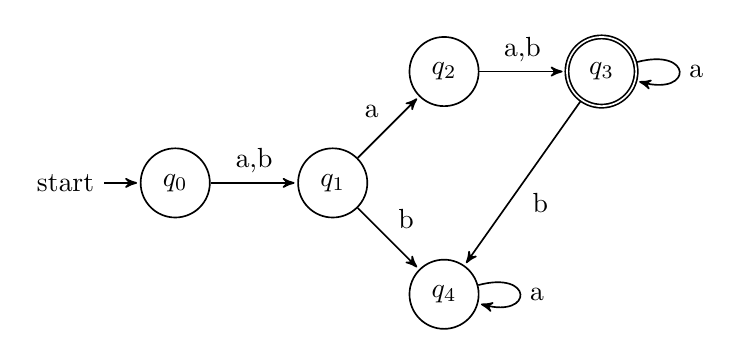
\begin{tikzpicture}[->,>=stealth',shorten >=1pt,auto,node distance=2cm,
	                    semithick]
	  \tikzstyle{every state}=[fill=none,draw=black,text=black]

	  \node[initial,state] (A)              {$q_0$};
	  \node[state]         (B) [right of=A] {$q_1$};
	  \node[state]         (C) [above right of=B] {$q_2$};
		\node[state, accepting] (D) [right of=C] {$q_3$};
		\node[state]         (E) [below right of=B] {$q_4$};

		\path (A) 	edge node {a,b} (B)
					(B)				edge node {a} (C)
	            			edge node {b} (E)
					(C) 			edge node {a,b} (D)
					(D) 		edge [loop right] node {a} (D)
	            			edge node {b} (E)
					(E)				edge [loop right] node {a} (E);
	\end{tikzpicture}
	\item Automat $M$ mit $L_3=T(M)=\set{(ab)^n}{n\in\N_0}$:\\

	\vspace{1em}
	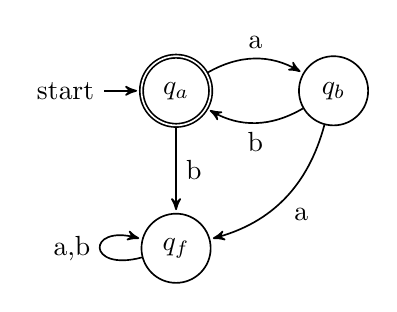
\begin{tikzpicture}[->,>=stealth',shorten >=1pt,auto,node distance=2cm,
	                    semithick]
	  \tikzstyle{every state}=[fill=none,draw=black,text=black]

	  \node[initial,state,accepting] (A)                    {$q_a$};
	  \node[state]         (B) [right of=A] {$q_b$};
	  \node[state]         (C) [below of=A] {$q_f$};

	  \path (A) edge [bend left]  node {a} (B)
	            edge              node {b} (C)
	        (B) edge [bend left]  node {b} (A)
	            edge [bend left]  node {a} (C)
	        (C) edge [loop left]  node {a,b} (C);
	\end{tikzpicture}

	\item Automat erkennt die Sprache

	$L_3=\set{w\in\simpleset{a,b,c}^\star}{w \text{ enthält das Teilwort $abc$ aber nicht das Teilwort $ab$}}$:

	\vspace{1em}
	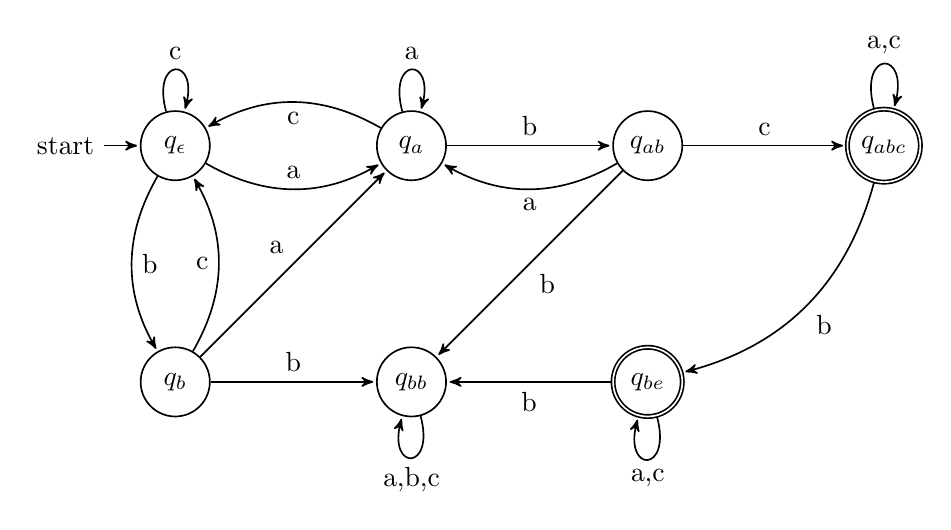
\begin{tikzpicture}[->,>=stealth',shorten >=1pt,auto,node distance=3cm,
	                    semithick]
	  \tikzstyle{every state}=[fill=none,draw=black,text=black]

	  \node[initial,state]   (Epsilon)   {$q_\epsilon$};
	  \node[state]           (A) [right of=Epsilon] {$q_a$};
	  \node[state]           (AB) [right of=A] {$q_{ab}$};
		\node[state, accepting](ABC) [right of=AB] {$q_{abc}$};
		\node[state]           (B) [below of=Epsilon] {$q_b$};
		\node[state]           (BB) [right of=B] {$q_{bb}$};
		\node[state, accepting](BE) [right of=BB] {$q_{be}$};

	  \path (Epsilon) edge [loop above] node {c} (Epsilon)
	            			edge [bend right] node {a} (A)
										edge [bend right] node {b} (B)
					(A)				edge [loop above] node {a} (A)
	            			edge              node {b} (AB)
										edge [bend right] node {c} (Epsilon)
					(AB) 			edge [bend left]  node {a} (A)
	            			edge              node {b} (BB)
										edge              node {c} (ABC)
					(ABC) 		edge [loop above] node {a,c} (ABC)
	            			edge [bend left]  node {b} (BE)
					(B)				edge              node {a} (A)
										edge              node {b} (BB)
										edge [bend right] node {c} (Epsilon)
					(BB)			edge [loop below] node {a,b,c} (BB)
					(BE)			edge [loop below] node {a,c} (ABC)
										edge              node {b} (BB);
	\end{tikzpicture}
\end{itemize}

	\chapter{Deterministisch kontextfreie Sprachen}
\begin{equation*}
	\dcfl\subset\cfl\subset\csl\subset\rec\subset\re
\end{equation*}

\section{Automatenmodell DPDA:}\label{dcfl:dpda}
Der deterministische Kellerautomat ist ähnlich definiert wie ein der nichtdeterministische (Siehe \autoref{cfl:pda}).

Der Unterschied zum PDA liegt dabei, dass beim DPDA in jeder Situation nur ein Übergang möglich sein darf,
\begin{equation*}
	\forall z\in Z, a\in\Sigma, A\in\Gamma : |\delta(z,a,A)|+|\delta(z,\epsilon,A)|\leq 1
\end{equation*}
und der DPDA akzeptiert nicht durch leeren Keller sondern durch Endzustände.

\paragraph{Ein deterministischer Kellerautomat ist ein 7-Tupel}
\begin{equation*}
	M=(Z,\Sigma,\Gamma,\delta,z_0,\#, E)
\end{equation*}
\begin{description}
	\item[$Z$] endliche Zustandsmenge
	\item[$\Sigma$] Eingabealphabet
	\item[$\Gamma$] Kelleralphabet
	\item[$\delta$] Überführungsfunktion $\delta:Z\times(\Sigma\cup\simpleset\epsilon)\times\Gamma \rightarrow Z\times\Gamma^\star$
	\item[$z_0$] Startzustand, $z_0\in Z$
	\item[$\#$] Keller-Bottom-Symbol $\#\in \Gamma\setminus\simpleset\Sigma$
	\item[$E$] Endzustandsmenge $E\subseteq Z$
\end{description}

\paragraph{Akzeptierte Sprache eines deterministischen PDA:}
\begin{equation*}
	N(M)\coloneqq\set{w\in \Sigma^\star}{\exists e\in E, V\in \Gamma^\star: (z_0, w, \#)\vdash^\star (e,\epsilon,V)}
\end{equation*}
dies wird auch als \emph{Akzeptieren durch Endzustand} bezeichnet.

Beide Akzeptanzarten, (durch Endzustand und leeren Keller, siehe \autoref{cfl:pda}) sind äquivalent.


\section{Sätze zu $\dcfl$:}
\begin{itemize}
	\item Eine deterministisch kontextfreie Sprache geschnitten mit einer regulären Sprache ist wieder eine deterministisch kontextfreie Sprache.
	\begin{equation*}
		L_1\in\dcfl, L_2\in\reg \Rightarrow L_1\cap L_2\in\dcfl
	\end{equation*}
	\item Die Klasse der deterministisch kontextfreien Sprachen ist nur abgeschlossen unter Komplement.
	\item Das Leerheitsproblem (Markieren von produktiven Variablen), das Wortproblem (in Linearzeit mit Kellerautomat) und das Äquivalenzproblem sind entscheidbar.

	Zum Äquivalenzproblem:
	\begin{align*}
		L=L'&\Leftrightarrow L\subseteq L' \wedge L'\subseteq L\\
				&\Leftrightarrow L\cap \overline{L'} = \emptyset \wedge L'\cap \overline L=\emptyset
	\end{align*}
	entscheidbar, da Abschluss unter Komplement und Leerheitsproblem entscheidbar.
\end{itemize}


\section{Beispiele: }
\begin{itemize}
	\item $L_1=\set{w\$w^R}{w\in\Sigma^\star}$ (markierte Palindrome)
	\item Deterministischer Kellerautomat, der die Sprache $L_2=\set{a^nb^n}{n\geq 1}$ akzeptiert:

	\vspace{1em}
	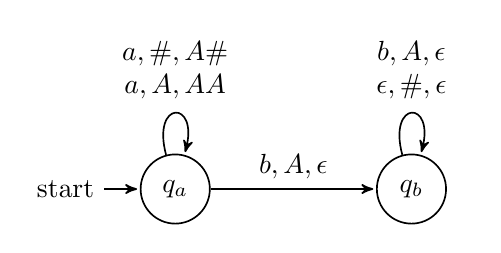
\begin{tikzpicture}[->,>=stealth',shorten >=1pt,auto,node distance=3cm,
	                    semithick]
	  \tikzstyle{every state}=[fill=none,draw=black,text=black]

	  \node[initial,state] 	(A)              {$q_a$};
	  \node[state]         	(B) [right of=A] {$q_b$};

	  \path (A) edge [loop above] node {\begin{tabular}{c}$a,\#,A\#$\\$a,A,AA$ \end{tabular}} (A)
	            edge              node {$b,A,\epsilon$} (B)
	        (B) edge [loop above] node {\begin{tabular}{c}$b,A,\epsilon$\\$\epsilon,\#,\epsilon$ \end{tabular}} (B);
	\end{tikzpicture}

	Konfigurationsübergänge bei Eingabewort $aaabb$:%
	\begin{align*}
		(z_a,aaabb,\#)&\vdash(z_a,aabb,A\#)\\
									&\vdash(z_a,abb,A\#)\\
									&\vdash(z_a,bb,AAA\#)\\
									&\vdash(z_a,b,AA\#)\\
									&\vdash(z_a,\epsilon,A\#)\\
									&\rightsquigarrow aaabb \not\in N(M)=L_2
	\end{align*}
\end{itemize}

	\chapter{Kontextfreie Sprachen $\cfl$: Typ-2}
\begin{equation*}
	\cfl\subset\csl\subset\rec\subset\re
\end{equation*}
Wort- und Leerheitsproblem entscheidbar.

Beschreib- und erkennbar durch einen nichtdeterministischen Kellerautomaten (PDA).
\section{Automatenmodell PDA:}


\section{Sätze zu den kontextfreien Sprachen:}
\begin{itemize}
	\item Jede kontextfreie Sprache über einem unären Alphabet ist regulär!
	\item Die Klasse der kontextfreien Sprachen ist abgeschlossen unter Sternoperation, Vereinigung und Konkatenation.
	\item Das Wortproblem ($\mathcal O(n^3)$) sowie das Leerheitsproblem sind entscheidbar.
\end{itemize}
\subsection{Pumping-Lemma für Typ-2:}
Sei $L\subseteq \Sigma^\star$ eine kontextfreie Sprache, dann gibt es eine Zahl $n$ so, dass für alle $z\in L$ mit $|z|\geq n$ eine Zerlegung mit $z=uvwxy$ in $u,v,w,x,y\in\Sigma^\star$ exisitert für die die drei Bedingungen erfüllt sind:
\begin{itemize}
	\item $|vx|\geq 1$
	\item $|vwx|\leq n$
	\item $\forall i\in N: uv^iwx^iy\in L$
\end{itemize}


\section{Chomsky-Normalform}
Eine Typ-2 Grammatik $(V,\Sigma,P,S)$ ist in Chomsky-Normalform (CNF),  wenn gilt:
\begin{equation*}
	\forall (u,v)\in P: v\in V^2\cup \Sigma
\end{equation*}
Zu jeder Typ-2 Grammatik existiert eine Grammatik $G'$ in CNF für die gilt $L(G)=L(G')$!
\subsection{Umformungsalgorithmus:}
\begin{enumerate}
	\item Zunächst wollen wir erreichen, dass folgendes gilt: $(u,v)\in P\Rightarrow (|v|>1 \vee v\in \Sigma)$
	\begin{enumerate}
		\item \textbf{Ringableitungen entfernen:}

		Eine Ringableitung liegt vor, wenn es Variablen $A_1,\ldots A_r$ gibt, die sich im Kreis in einander ableiten lassen, d.h. es gibt Regeln $A_i\rightarrow A_{i+1}$ und $A_r\rightarrow A_1$.

		Um dies loszuwerden, werden alle Variablen $A_i$ durch eine neue Variable $A$ ersetzt. Überflüssige Regeln wie $A\rightarrow A$ werden gelöscht.
		\item \textbf{Variablen anordnen:}

		Man legt eine Ordnung der Variablen fest: $V=\simpleset{B_1, B_2, \ldots, B_n}$, hierfür muss gelten:
		\begin{equation*}
			A_i\rightarrow A_j \in P \Leftrightarrow i<j
		\end{equation*}
		Falls dies nicht gilt, müssen Abkürzungen verwendet werden, also alle Produktionen von $A_j$ werden eingesetzt:
		\begin{equation*}
			P=(P\setminus\simpleset{A_i\rightarrow A_j})\cup\set{(A_i,w)}{(A_j,w)\in P}
		\end{equation*}
	\end{enumerate}
	\item Jetzt gilt für jede Regel $(u,v)\in P$ entweder $v\in\Sigma$ oder $|v|\geq 2$.

	Für letztere Regeln werden nun Pseudoterminale eingeführt. Es werden neue Variablen und Produktionen für jedes Terminalsymbol hinzugefügt, z.B. $V_a\rightarrow a$.

	\item \textbf{Letzer Schritt:} Alle rechten Seiten mit $|v|>2$ müssen nun noch auf Länge 2 gekürzt werden. Hierfür werden wiederum neue Variablen eingefügt:%
	\begin{align*}
		A\rightarrow C_1C_2C_3\\
		\intertext{Wird gekürzt zu}
		A\rightarrow C_1D_1\\
		D_1\rightarrow C_2C_3
	\end{align*}
\end{enumerate}

\section{Greibach-Normalform}
Eine Typ-2 Grammatik $(V,\Sigma,P,S)$ ist in Greibach-Normalform (GNF),  wenn gilt:
\begin{equation*}
	\forall (u,v)\in P: v\in \Sigma V^\star
\end{equation*}
Zu jeder Typ-2 Grammatik existiert eine Grammatik $G'$ in GNF für die gilt $L(G)=L(G')$!
\subsection{Umformungsalgorithmus:}
\begin{enumerate}
	\item \textbf{Mh?}

	\item \textbf{Beseitigung von Linksrekursion:}

	Alle Produktionsregeln sind von der Form:
	\begin{align*}
		A&\rightarrow A\alpha_1|\ldots|A\alpha_k|\beta_1|\ldots|\beta_l\\
		\intertext{Diese können durch diese $2k+2l$ Regeln ersetzt werden:}
		A&\rightarrow \beta_1|\ldots|\beta_l\\
		A&\rightarrow \beta_1B|\ldots|\beta_lB\\
		B&\rightarrow \alpha_1|\ldots|\alpha_k\\
		B&\rightarrow \alpha_1B|\ldots|\alpha_kB
	\end{align*}%
	Nun sind keinerlei Linksrekursionen mehr vorhanden!
\end{enumerate}

\section{Beispiele: }
\begin{itemize}
	\item $L_1=\set{a^nb^n}{n\geq 1}$ (zwei gleiche Exponenten)
	\item $L_2=\set{ww^R}{w\in\Sigma^\star}$ (unmarkierte Palindrome)
	\item Korrekt geklammerte arithmetische Ausdrücke (Dyck-Wörter)
\end{itemize}

	\chapter{Kontextsensitive Sprachen $\csl$: Typ-1}
\begin{equation*}
	\csl\subset\rec\subset\re
\end{equation*}
Wortproblem entscheidbar. Abschluss unter allen Operationen.

\section{Algorithmus zur Entscheidbarkeit des Wortproblems:}
Die Funktion $\mathrm{Abl}_n(X)$ wird iteriert angewendet, bis sich entweder $X$ nicht mehr ändert ($w\not\in L(G)$) oder das gesuchte Wort $w$ in $X$ enthalten ist ($w\in L(G)$).

Dabei ist $n$ die Länge des gesuchten Worts $w$, also $|w|$.

Die Funktion $\mathrm{Abl}_n(X)$ ist für eine Grammatik $G$ wie folgt definiert:
\begin{equation*}
	\mathrm{Abl}_n(X)\coloneqq X\cup\set{w\in(V\cup\Sigma)^\star}{|w|\leq n \wedge \exists y\in X:y\Rightarrow_G w}
\end{equation*}


\section{Automatenmodell LBA:}
Die Kontextsensitiven Sprachen werden von linear beschränkten Automaten akzeptiert.



\section{Beispiele: }
\begin{itemize}
	\item $L_1=\set{a^nb^nc^n}{n\geq 1}$ (drei und mehr gleiche Exponenten)
	\item
\end{itemize}


\part{Berechenbarkeitstheorie und Komplexität}
	\chapter{Rekursiv aufzählbare Sprachen}\label{sec:typ0}
\begin{equation*}
	\operatorname{Typ-0} = \re
\end{equation*}



Eine Turingmaschine $M$ \emph{akzeptiert} die Sprache $L$, wenn sie nach endlicher Zeit hält.
Bei Eingaben, die nicht zu $L$ gehören, rechnet sie unendlich lang weiter (dieses Verhalten führt später auf das Halteproblem).
Solche Sprachen $L$ gehören dann zu $\re$, sie sind \emph{semi-entscheidbar}.



\section{Sätze zu $\re$}
\begin{itemize}
	\item Die Klasse der Typ-0 Sprachen ist abgeschlossen unter Sternopertaion, Vereinigung, Schnitt und Konkatenation.
	\item Die Klasse der durch Turingmaschinen erkennbaren/akzeptierten Sprachen ist gleich der Klasse der rekursiv aufzählbaren.
\end{itemize}

	\chapter{Entscheidbare Sprachen $\rec$:}
\begin{equation*}
	\rec\subset\re
\end{equation*}

	\chapter{Berechenbarkeitstheorie}
\begin{center}
	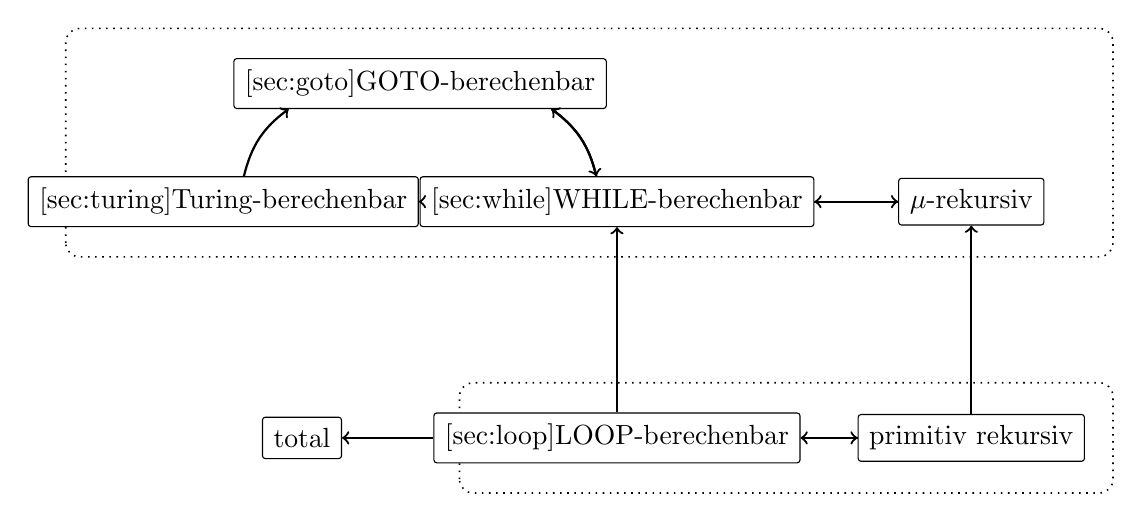
\begin{tikzpicture}
		\tikzset{
			grouplabel/.style={
				draw,
				fill = white,
				rectangle,
				inner sep = 4pt,
				rounded corners=1pt
			}
		}

		\draw [rounded corners=5pt, dotted, line width=0.2mm] (0,6.3) rectangle (13.3,9.2);
		\draw node (tm) at (2,7) [grouplabel] {\hyperref[sec:turing]{Turing-berechenbar}};
		\draw node (while) at (7,7) [grouplabel] {\hyperref[sec:while]{WHILE-berechenbar}};
		\draw node (goto) at (4.5,8.5) [grouplabel] {\hyperref[sec:goto]{GOTO-berechenbar}};
		\draw node (mu) at (11.5,7) [grouplabel] {$\mu$-rekursiv};
		\draw [rounded corners=5pt, dotted, line width=0.2mm] (5,3.3) rectangle (13.3,4.7);
		\draw node (loop) at (7,4) [grouplabel] {\hyperref[sec:loop]{LOOP-berechenbar}};
		\draw node (prek) at (11.5,4) [grouplabel] {primitiv rekursiv};
		\draw node (total) at (3,4) [grouplabel] {total};

		\draw[thick, ->] (while) to (tm);
		\draw[thick, ->] (tm) to[bend left=20] (goto);
		\draw[thick, ->] (goto) to[bend left=20] (while);
		\draw[thick, ->] (while) to[bend right=20] (goto);
		\draw[thick, ->] (mu) to (while);
		\draw[thick, ->] (while) to (mu);

		\draw[thick, ->] (prek) to (mu);
		\draw[thick, ->] (loop) to (while);
		\draw[thick, ->] (loop) to (prek);
		\draw[thick, ->] (prek) to (loop);

		\draw[thick, ->] (loop) to (total);
	\end{tikzpicture}
\end{center}




\section{LOOP-Berechenbarkeit}\label{sec:loop}
Eine Funktion $f:\N^k\rightarrow \N$ heißt LOOP-berechenbar,  falls es ein LOOP-Program $P$ gibt, das gestartet auf der Eingabe $n_1,n_2,\ldots,n_k$ in den Variablen $x_1,x_2,\ldots,x_n$ nach endlich vielen Schritten hält und die Variable $x_0$ den Wert $f(n_1,\ldots,n_k)$ beinhaltet.
\subsection{Erlaubte Basisanweisungen}
\begin{itemize}
	\item $x_i\coloneqq x_j+c$ bzw. $x_i\coloneqq x_j-c$ mit $c\in\N$
	\item LOOP $x_i$ DO $P$ END
	\item Hintereinanderausführung
\end{itemize}
\subsection{Simulierbare Makros}
\begin{itemize}
	\item Wertzuweisungen $x_i\coloneqq x_j$ und $x_i\coloneqq c$
	\item IF $x_i>c$ THEN $P$ END
	\item Übliche Arithmetische Operationen (Multiplikation und Division), sogar $\mathrm{mod}$
\end{itemize}

\section{WHILE-Berechenbarkeit}\label{sec:while}
Eine Funktion $f:\N^k\rightarrow \N$ heißt WHILE-berechenbar,  falls es ein WHILE-Program $P$ gibt, das gestartet auf der Eingabe $n_1,n_2,\ldots,n_k$ in den Variablen $x_1,x_2,\ldots,x_n$ nach endlich vielen Schritten hält (falls das Ergebnis definiert ist) und die Variable $x_0$ den Wert $f(n_1,\ldots,n_k)$ beinhaltet. Ist $f(n_1,\ldots,n_k)$ undefiniert, so hält $P$ nicht.
\subsection{Erlaubte Anweisungen}
\begin{itemize}
	\item In WHILE-Programmen sind alle Anweisungen von LOOP-Programmen erlaubt sowie die WHILE-Schleife:

	\item WHILE $x_i\neq 0$ DO $P$ END
\end{itemize}


\section{GOTO-Berechenbarkeit}\label{sec:goto}
\subsection{Erlaubte Anweisungen}
\begin{itemize}
	\item Berechnungen und Zuweisungen: $x_i\coloneqq x_j\pm c$
	\item Marken: $M_i$
	\item GOTO $M_i$
	\item HALT
	\item IF $x_i=c$ THEN GOTO $M_j$
\end{itemize}

\section{Turing-Berechenbarkeit}\label{sec:turing}
Eine Funktion $f:\N^k\rightarrow \N$ heißt Turing-berechenbar, falls eine deterministische Turingmaschine existiert, die $f(n_1,\ldots,n_k)=m$ berechnet indem, sie gestartet auf dem $k$-Tupel $(n_1,\ldots,n_k)$ nach endlich vielen Berechnungsschritten einen Endzustand erreicht und dann $m$ auf dem Band steht. Falls das Ergebnis für die Eingabe undefiniert ist, terminiert die Maschine nie.

\section{Primitive Rekursion}
Eine Funktion ist genau dann primitiv rekursiv, wenn sie LOOP-berechenbar ist.
\begin{itemize}
	\item Konstante Funktionen sind primitiv rekursiv
	\item Projektionen sind primitiv rekursiv
	\item Die Nachfolgerfunktion $s:\N\rightarrow\N, n\mapsto n+1$ ist primitiv rekursiv
	\item Verkettungen von primitiv rekursiven Funktionen sind primitiv rekursiv
	\item Funktionen, die durch primitive Rekursion aus primitiv rekursiven Funktionen entstehen, sind primitiv rekursiv:
	\begin{align*}
		f(0,x_1,\ldots,x_k)&=g(x_1,\ldots,x_k)\\
		f(n+1,x_1,\ldots,x_k)&=h(f(n,x_1,\ldots,x_k),n,x_1,\ldots,x_k)
	\end{align*}
	Das heißt, $g, h$ primitiv rekursiv $\Rightarrow$ $f$ primitiv rekursiv.
\end{itemize}
\subsection{Beispiele für primitiv rekursive Funktionen:}
\begin{itemize}
	\item Cantor'sche Paarungsfunktion
	\begin{align*}
		&c(x,y)=\binom{x+y+1}{2}+x \quad\text{ (bijektiv)}
		\intertext{mit den Umkehrungsfunktionen}
		&e(c(x,y))=x\text{ und }f(c(x,y))=y
	\end{align*}
	\item
\end{itemize}

\section{$\mu$-Rekursion}
\begin{equation*}
	\mu f(x_1,\ldots,x_k)=\min \set{n\in\N}{f(n,x_1,\ldots,x_k)=0 \wedge \forall m<n:f(m,x_1,\ldots,x_k)>0}
\end{equation*}
Der $\mu$-Operator liefert den kleinsten Eingabewert $n$ der ersten Variable, bei der die Funktion $0$ ausgibt. Dabei muss insbesondere $f$ für alle Werte kleiner als $n$ definiert sein, da sonst eine Berechnung nicht möglich wäre.

\begin{satz}{Satz von Kleene}
	Sei $f:\N^n\rightarrow\N$ eine $\mu$-rekursive Funktion. Dann existieren zwei $(n+1)$-stellige primitiv rekursive Funktionen $p$ und $q$ mit
	\begin{equation*}
		f(x_1,\ldots,x_n)=p(x_1,\ldots,x_n,\mu q(x_1,\ldots,x_n))
	\end{equation*}
\end{satz}

	%!TEX root = ../main.tex
\chapter{Entscheidbarkeitstheorie}
Die Berechenbarkeitstheorie spielt sich innerhalb der Entscheidbarkeitstheorie ab. Wenn eine Sprache entscheidbar ist, macht es Sinn ihre Komplexität zu bestimmen. Andersherum heißt das, dass jede Sprache, die in einer der Komplexitätsklassen enthalten ist entscheidbar ist (also insbesondere semi- und co-semi-entscheidbar).

\section{Definitionen}
\subsection{Charakteristische Funktionen}
Für jede Menge $A$ existiert die sogenannte \emph{charakteristische Funktion} $\chi_A(w)$. Diese Funktion entscheidet für jedes Wort $w$ aus einer festgelegten Grundmenge, ob $w\in A$ gilt.
\begin{equation*}
	\chi_A(w)=\begin{cases}
		1\text{, falls } w\in A\\
		0\text{, sonst}
	\end{cases}
\end{equation*}

Ebenso lässt sich die semi-charakteristische Funktion $\chi_A'(w)$ definieren
\begin{equation*}
	\chi_A'(w)=\begin{cases}
		1\text{, falls } w\in A\\
		\mathrm{undefiniert}\text{, sonst}
	\end{cases}
\end{equation*}

Eine Menge heißt \emph{entscheidbar}, wenn ihre zugehörige charakteristische Funktion \emph{berechenbar} ist. Eine Menge heißt semi-entscheidbar, falls die semi-charakteristische Funktion berechenbar ist. Das Komplement einer Mengen, deren semi-charakteristische Funktion berechenbar ist, heißt co-semi-entscheidbar.

Ist eine Menge entscheidbar, so ist es ihr Komplement trivialerweise auch.

\subsection{Rekursive Aufzählbarkeit}
Eine Sprache $A$ ist rekursiv aufzählbar, wenn eine totale, berechenbare Funktion $c:\N\rightarrow\Sigma^\star$ existiert sodass $A=\set{c(n)}{n\in\N}$ gilt. Rekursive Aufzählbarkeit ist äquivalent zu Semi-Entscheidbarkeit.

\subsection{Entscheidbarkeitsprobleme}
Hierbei seien die Gödelisierungen der Maschinen in einer geeigneten Art und Weise kodiert. Beispielsweise $w\in\simpleset{0,1}^\star$ für eine Maschine $M_w$.
\medskip

\begin{tabular}{r|c|l}
	Spezielles Halteproblem & $K=\set{w}{M_w \text{ hält auf Eingabe } w}$ & semi-entscheidbar\\
	Allgemeines Halteproblem & $H=\set{w\# x}{M_w \text{ hält auf Eingabe } x}$ & semi-entscheidbar\\
	Halteproblem auf leerem Band & $H_0=\set{w}{M_w \text{ hält auf Eingabe } \epsilon}$ & semi-entscheidbar\\
	PCP & Postsches Korrespondenzproblem & semi-entscheidbar\\
	MPCP & Für alle Lösungen gilt $i_1=1$ & semi-entscheidbar\\
	WA & Menge aller wahren arithmetischen Formeln & unentscheidbar\\
	$\overline{\text{WA}}$ & Menge aller falschen arithm. Formeln & unentscheidbar
\end{tabular}

\paragraph{Satz von Rice}
Sei $\mathcal R$ die Klasse der Turing-berechenbaren Funktionen und $\mathcal S$ eine nichttriviale Teilmenge von $\mathcal R$.
Dann ist die Menge $C(\mathcal S)=\set{w}{M_w \text{ berechnet eine Funktion aus } \mathcal S}$ unentscheidbar.

Wichtig ist, dass der Satz von Rice nur Aussagen über berechnete Funktionen macht, Aussagen über die berechnende Turingmaschine werden nicht in Betracht gezogen.

Bei der Verwendung des Satzes von Rice führt man eigentlich eine \hyperref[sec:reduktion]{Reduktion} durch, muss sich jedoch keine Funktion mehr einfallen lassen.

\paragraph{Probleme in der Theorie der formalen Sprachen}
\begin{itemize}
	\item Für deterministisch kontextfreie Sprachen $L,K\in\dcfl$ sind die Fragen $L\cap K=\emptyset$, $|L\cap K|<\infty$, $L\cap K \in \cfl$ sowie $L\subseteq K$ unentscheidbar.
	\item Für eine kontextfreie Grammatik sind die Frage nach Mehrdeutigkeit, $\overline{L(G)}\in\cfl$, $L(G)\in \reg$ und $L(G)\in \dcfl$ alle unentscheidbar.
	\item Für eine kontextsensitive-Grammatik ist die Leerheit sowie die Endlichkeit der erzeugten Sprache unentscheidbar.
\end{itemize}

\section{Reduktion von Problemen}\label{sec:reduktion}
Um die prinzipielle Lösbarkeit zweier Probleme zu betrachten, verwendet man Reduktionen:

Seien $A\subseteq \Sigma^\star$ und $B\subseteq \Gamma^\star$ zwei Probleme. Kann man eine \emph{totale und berechenbare Funktion} $f:\Sigma^\star\rightarrow\Gamma^\star$ finden, so dass gilt
\begin{equation*}
	x\in A\Leftrightarrow f(x)\in B,
\end{equation*}
so sagt man, $A$ ist auf $B$ (many-one-)reduzierbar.
Man schreibt dann auch $A\leq B$.

\begin{enumerate}
	\item $A\leq B$ und $B$ entscheidbar $\Rightarrow$ $A$ entscheidbar.
	\item $A\leq B$ und $B$ semi-entscheidbar $\Rightarrow$ $A$ semi-entscheidbar.
\end{enumerate}

Bei der Reduktion übertragen sich immer fehlende Eigenschaften von links nach rechts, d.h. reduziert man ein semi-entscheidbares, aber nicht co-semi-entscheidbares Problem $A$ auf ein Problem $B$ (d.h. $A\leq B$), so ist $B$ ebenfalls nicht co-semi-entscheidbar. Über die Semi-Entscheidbarkeit von $B$ wird keine Aussage gemacht.

Reduziert man allerdings ein unbekanntes Problem $A$ auf ein semi-entscheidbares Problem $B$ (d.h. $A\leq B$), so hat man die Semi-Entscheidbarkeit von $A$ gezeigt. Es übertragen sich also \glqq positive Eigenschaften\grqq\  von rechts nach links.

Letzterer Sachverhalt wird klar, wenn man sich überlegt, dass man mit der Reduktion eine Funktion gefunden hat, die eine Fragestellung aus $A$ in eine aus $B$ überträgt. Man kann also das Entscheidungsproblem für $A$ zunächst in $B$ übersetzen und schließlich mit dem Entscheidungsalgorithmus für $B$ entscheiden.

\paragraph{Beispiel einer Reduktion:}
Wir wollen zeigen, dass die Sprache
$$L=\set{w\in\simpleset{0,1}^\star}{T(M_w)\in\reg}$$
das heißt die Menge der Turingmaschinen, die reguläre Sprachen akzeptieren, unentscheidbar ist. Dafür reduzieren wir $H_0\leq L$, dabei sei $f(w)$ die Kodierung einer Turingmaschine die auf Eingabe $x$ wie folgt arbeitet
\begin{itemize}
	\item Wenn die Eingabe von der Form $x=a^nb^n$ mit $n\in\N$ ist, akzeptiere.
	\item Sonst lösche die Eingabe und simuliere $M_w$ auf leerem Band.
\end{itemize}
Hierbei sei die Maschine o.B.d.A. über einem Alphabet $\simpleset{a,b}\subset\Sigma$ definiert.
Damit ist $f$ total und berechenbar und es gilt
\begin{align*}
	w\in H_0&\Rightarrow T(M_{f(w)})=\Sigma^\star & w\not\in H_0&\Rightarrow T(M_{f(w)})=\set{a^nb^n\in\Sigma^\star}{n\in\N}\\
	&\Rightarrow T(M_{f(w)})\in\reg&&\Rightarrow T(M_{f(w)})\in\cfl\setminus\reg 
\end{align*}
Da $H_0$ unentscheidbar ist, ist es auch $L$.\hfill$\Box$
	\chapter{Komplexitätstheorie}
Die Frage in der Komplexitätstheorie ist, wie viel Aufwand benötigt wird, ein Problem zu lösen.
Die theoretische Lösbarkeit wird in der Entscheidbarkeits- bzw. Berechenbarkeitstheorie behandelt.

Die Komplexitätstheorie befasst sich mit oberen und unteren Schranken an den Ressourcenaufwand zur Problemlösung.
Wichtig sind hierbei auch inhärente Komplexitäten, also eine Beschränkung nach oben und unten.
\section{Komplexitätsklassen}
Diese Komplexitätsklassen liegen alle in der Menge der entscheidbaren Sprachen. Alle folgenden Klassen sind also Teilmengen von $\rec$.

Für alle Komplexitätsklassen $\mathcal C$ ist zu unterscheiden:
\begin{align*}
	\operatorname{co}\mathcal C=\set{L\in\Sigma^\star}{\overline L \in\mathcal C} && \overline{\mathcal C}=\set{L\in\Sigma^\star}{L\not\in \mathcal C}
\end{align*}
\subsection{Zeitklassen}
\begin{multicols}{2}
	Die Funktion $\mathrm{time}_M:\Sigma^\star\rightarrow \N$ ordnet einer Eingabe die Anzahl Schritte zu, die eine deterministische Maschine $M$ auf ihr ausführt.

	Die Zeitklasse $\operatorname{DTIME}(f(n))$ enthält alle Probleme, die sich durch eine deterministische Turingmaschine in einem Zeitaufwand kleiner als $f$ lösen lassen. Das heißt, $f$ ist eine obere Schranke für die Komplexität der Probleme in $\operatorname{TIME}(f)$.

	\columnbreak

	Die Funktion $\mathrm{ntime}_M:\Sigma^\star\rightarrow \N$ ordnet einer Eingabe die Länge des kürzesten akzeptierenden Pfades der nichtdeterministischen Maschine $M$ zu. Falls die Maschine nicht akzeptiert, ist $\mathrm{ntime}_M(w)=0$.

	Die Zeitklasse $\operatorname{NTIME}(f(n))$ enthält alle Probleme, die sich durch eine nichtdeterministische Turingmaschine in einem Zeitaufwand kleiner als $f$ lösen lassen.
\end{multicols}



\begin{center}
	\renewcommand{\arraystretch}{2}
	\begin{tabular}{rl}
		\poly&$=\displaystyle\bigcup_{k\geq 1} \operatorname{DTIME}(n^k)$\\
		\npoly&$=\displaystyle\bigcup_{k\geq 1} \operatorname{NTIME}(n^k)$
	\end{tabular}
\end{center}

\subsection{Platzklassen}
Analog zu den Zeitklassen sind Platzklassen definiert, die den maximal belegten Platz für eine Berechnung beschränken. Die Funktion $\mathrm{space}_M:\Sigma^\star\rightarrow \N$ ordnet dabei jeder Eingabe auf einer deterministischen Turingmaschine die Anzahl der maximal verwendeten Bandelemente (auf einem Arbeitsband) zu.

So ist die Platzklasse $\operatorname{SPACE}(f(n))$ definiert als die Klasse aller Probleme für die $f$ eine Platzbeschränkung für alle Eingaben ist.

Analog wie bei Zeitklassen die Unterscheidung deterministische-nichtdeterministische Platzklassen.
\begin{center}
	\renewcommand{\arraystretch}{2}
	\begin{tabular}{rl}
		\textbf{L}&$=\operatorname{DSPACE}(\log)$\\
		\textbf{NL}&$=\operatorname{NSPACE}(\log)$\\
		\textbf{PSPACE}&$=\displaystyle\bigcup_{k\geq 1} \operatorname{DSPACE}(n^k)=\bigcup_{k\geq 1} \operatorname{NSPACE}(n^k)$
	\end{tabular}
\end{center}

\subsection{Wichtige Beziehungen zwischen den Klassen}
\begin{itemize}
	\item In den Platzklassen spielt die $\mathcal O$-Notation keine Rolle, Konstanten können wegen Bandreduktion und Bandkompression vernachlässigt werden
	\begin{align*}
		\operatorname{DSPACE}(\mathcal O(f))&=\operatorname{DSPACE}(f)\\
		\operatorname{NSPACE}(\mathcal O(f))&=\operatorname{NSPACE}(f)
	\end{align*}
	\item In nichtdeterministischen Zeitklassen spielt die $\mathcal O$-Notation ebenfalls keine Rolle
	\begin{equation*}
		\operatorname{NTIME}(\mathcal O(f))=\operatorname{NTIME}(f)
	\end{equation*}
	\item Bei deterministischen Zeitklassen gilt i.A. $\operatorname{DTIME}(\mathcal O(f))\not=\operatorname{DTIME}(f)$, nur für größer als lineare Funktionen gilt Gleichheit d.h.
	\begin{align*}
		\operatorname{DTIME}(\mathcal O(f))&=\operatorname{DTIME}(f) \enspace f(n)\geq (1+\epsilon)n\text{ für ein }\epsilon>0\\
		\operatorname{DTIME}(f)&\subseteq \operatorname{DTIME}(f\log f)
	\end{align*}
	\item Für alle $f(n)\geq n$ gilt für die Zeitklassen
	\begin{equation*}
		\operatorname{DTIME}(f)\subseteq\operatorname{NTIME}(f)\subseteq\operatorname{DSPACE}(f)
	\end{equation*}
	\item Und für alle $f(n)\geq \log n$ gilt
	\begin{equation*}
		\operatorname{DSPACE}(f)\subseteq\operatorname{NSPACE}(f)\subseteq\operatorname{DTIME}(2^{\mathcal O(f)})
	\end{equation*}
	\item \textbf{Satz von Savitch}: Sei $s\in\Omega(\log(n))$, dann gilt
	\begin{equation*}
		\operatorname{NSPACE}(s)\subseteq\operatorname{DSPACE}(s^2)
	\end{equation*}
	\item Sei $s_1\not\in\Omega(s_2)$ und $s_2\in\Omega(\log(n))$, dann gilt der \textbf{Platzhierarchiesatz}
	\begin{equation*}
		\operatorname{DSPACE}(s_2)\setminus\operatorname{DSPACE}(s_1)\not=\emptyset
	\end{equation*}
	\item Sei $t_1\log(t_1)\not\in\Omega(t_2)$ und $t_2\in\Omega(n\log(n))$, dann gilt der \textbf{Zeithierarchiesatz}
	\begin{equation*}
		\operatorname{DTIME}(t_2)\setminus\operatorname{DTIME}(t_1)\not=\emptyset
	\end{equation*}
	\item \textbf{Lückensatz von Borodin}: Für jede totale berechenbare Funktion $r(n)\geq n$ existiert effektiv eine totale berechenbare Funktion $s(n)\geq n+1$ mit
	\begin{equation*}
		\operatorname{DTIME}(s(n))=\operatorname{DTIME}(r(s(n)))
	\end{equation*}
	\item Translationtechnik:\\
	Die Translationssätze werden verwendet, Separationen von größeren zu kleineren Klassen bzw. Gleichheiten oder Inklusionen von kleineren zu größeren Klassen zu übertragen.
	Die durch Padding aufgebläte Sprache ist $Pad_f(L)\coloneqq \set{w\$^{f(|w|)-|w|}}{w\in L}$.
	\begin{enumerate}
		\item Für zwei Funktionen $f(n),g(n)\geq n$ gilt der \textbf{Translationssatz für Zeitklassen}:
		\begin{align*}
			Pad_f(L)\in \operatorname{DTIME}(\mathcal O(g))&\Leftrightarrow L\in \operatorname{DTIME}(\mathcal O(g\circ f))\\
			Pad_f(L)\in \operatorname{NTIME}(\mathcal O(g))&\Leftrightarrow L\in \operatorname{NTIME}(\mathcal O(g\circ f))
		\end{align*}
		\item Und analog für $g\in\Omega(\log)$ und $f(n)\geq n$ der \textbf{Translationssatz für Platzklassen}:
		\begin{align*}
			Pad_f(L)\in \operatorname{DSPACE}(\mathcal O(g))&\Leftrightarrow L\in \operatorname{DSPACE}(\mathcal O(g\circ f))\\
			Pad_f(L)\in \operatorname{NSPACE}(\mathcal O(g))&\Leftrightarrow L\in \operatorname{NSPACE}(\mathcal O(g\circ f))
		\end{align*}
	\end{enumerate}
\end{itemize}





\section{Reduktionen}
Ähnlich wie in der Berechenbarkeitstheorie kann man zur Analyse der Komplexität von Problemen Reduktionen zwischen diesen entwickeln. Hier ist das Ergebnis allerdings sogar eine Beschränkung des Aufwands nach oben oder unten.

Allerdings ist die many-one-Reduktion zu grob um sinnvolle Reduktionen zwischen Problemen mit Zeitbeschränkung durchzuführen. {\scriptsize(Ein Problem, das in Polynomialzeit lösbar ist, könnte durch eine many-one-Reduktionsfunktion gelöst werden. So kann man eigentlich alle berechenbaren Probleme aufeinander many-one-reduzieren, diese Aussage ist jedoch für eine Komplexitätsbetrachtung uninteressant.)}

Deshalb gibt es die sog. Polynomialzeitreduktion. Hier ist eine Beschränkung an die Reduktionsfunktion gesetzt, nämlich muss diese zusätzlich in Polynomialzeit berechenbar sein. Man schreibt $A\leq_p B$.
\begin{enumerate}
	\item $A\leq_p B\wedge B\in \text{\poly}\Rightarrow A\in\text{\poly}$
	\item $A\leq_p B\wedge B\in \text{\npoly}\Rightarrow A\in\text{\npoly}$
\end{enumerate}


\subsection{Härte und Vollständigkeit}
\paragraph{NP-Härte}
Eine Sprache ist \npoly-hart falls sich alle Probleme aus \npoly\ in Polynomialzeit darauf reduzieren lassen. Das heißt dieses Problem ist mindestens so schwierig zu lösen wie ein Problem aus \npoly. Es gilt: $A$ \npoly-hart und $A\leq_p B\Rightarrow B$ \npoly-hart.
\paragraph{NP-Vollständigkeit}
Ist eine Sprache \npoly-hart und selbst in \npoly\ enthalten, so nennt man sie \npoly-vollständig. Diese Sprachen gehören zu den schwierigsten Sprachen aus \npoly. Kann man von einer \npoly-vollständigen Sprache zeigen, dass sie sogar in \poly\ liegt, so hat man \poly$=$\npoly\ gezeigt.

Einige \npoly-vollständige Probleme:
\begin{center}
	\begin{tabular}{r|l}
		\textbf{SAT} & $\set{w}{w\text{ kodiert eine erfüllbare Formel}}$\\
		\textbf{3KNF-SAT} & Ist eine Formel in KNF mit max. 3 Literalen pro Klausel erfüllbar?\\
		\textbf{CLIQUE} & Enthält ein Graph eine Clique der Größe $k$?\\
		\textbf{FÄRBBARKEIT} & Gibt es eine Knotenfärbung mit $k$ Farben?\\
	\end{tabular}
\end{center}

\paragraph{PSPACE-Vollständigkeit}
\textbf{QBF} $=\set{F}{F\text{ ist eine geschlossene \textbf{QBF}-Formel, die sich zum Wert TRUE auswerten lässt.}}$ ist $\operatorname{PSPACE}$-vollständig.

\subsection{Logspace-Reduktion}
\paragraph{Logspace-Transducer}
Ein Logspace-Transducer ist eine deterministische Turingmaschine mit einem read-only Eingabeband und einem logarithmisch beschränkten Arbeitsband, sowie einem write-only Ausgabeband auf dem der Schreib-/ Lesekopf nicht nach links bewegt werden kann.

Eine Funktion heißt logspace-berechenbar, wenn ein Logspace-Transducer existiert, der sie berechnet.

Auf Basis dieser Definitionen gibt es nun als verfeinerung der Polynomialzeitreduktion die Logspace-Reduktion:

Seien $A,B\subseteq \Sigma^\star$ Sprachen. $A$ heißt auf $B$ logspace-reduzierbar, falls eine logspace-berechenbare Funktion $f:\Sigma^\star\rightarrow\Sigma^\star$ existiert, so dass
\begin{equation*}
	x\in A\Leftrightarrow f(x)\in B
\end{equation*}
Man schreibt dann $A\leq_{\log} B$.

So kann man nun Begriffe wie \textbf{NL}- bzw. \poly-Härte/-Vollständigkeit sinnvoll (und analog zur \npoly-Vollständigkeit) definieren.

Einige Probleme, die \textbf{NL}-vollständig bezüglich logspace-Reduktion sind:
\begin{center}
	\begin{tabular}{r|l}
		\textbf{GAP} & Grapherreichbarkeitsproblem\\
		\textbf{2-SAT} & erfüllbare boole'sche Formeln in 2KNF-Darstellung\\
		\textbf{2-NSAT} & nicht erfüllbare Formeln in 2KNF-Darstellung
	\end{tabular}
\end{center}

Einige Probleme, die \poly-vollständig bezüglich logspace-Reduktion sind:
\begin{center}
	\begin{tabular}{r|l}
		\textbf{CFE} & $L_{cfe}=\set{w}{w\text{ ist Kodierung einer Typ-2 Grammatik $G$ mit }L(G)=\emptyset}$\\
		\textbf{CVP} & Circuit Value Problem (Ausgabe des Schaltnetzes)\\
		\textbf{MCVP} & Wie \textbf{CVP}, allerdings ohne Negationen
	\end{tabular}
\end{center}



\end{document}
